% Domain grid visualisations (DST grid + interior degrees of freedom).
%
% Requires in the preamble:
%   \usepackage{amsmath}
%   \usepackage{graphicx}
%   \usepackage{subfig}
%   \usepackage{epstopdf}   % the figures are EPS; needed under pdflatex,
%                           % which then wants -shell-escape. Not needed for
%                           % latex/dvips, which reads EPS directly.
%
% The figures live next to this file, in results_paper/grid_visualisation/.
% If you \input this snippet from elsewhere, point graphicx at that folder, e.g.
%   \graphicspath{{results_paper/grid_visualisation/}}
% and drop the leading path from the \includegraphics arguments below.
%
% Excluded on purpose: the "square" and "small_rectangle" domains.

\begin{figure}[htbp]
  \centering
  \subfloat[Domain \texttt{rectangle}, $M = 49$, $\mathtt{DOF} = 1176$.]{%
    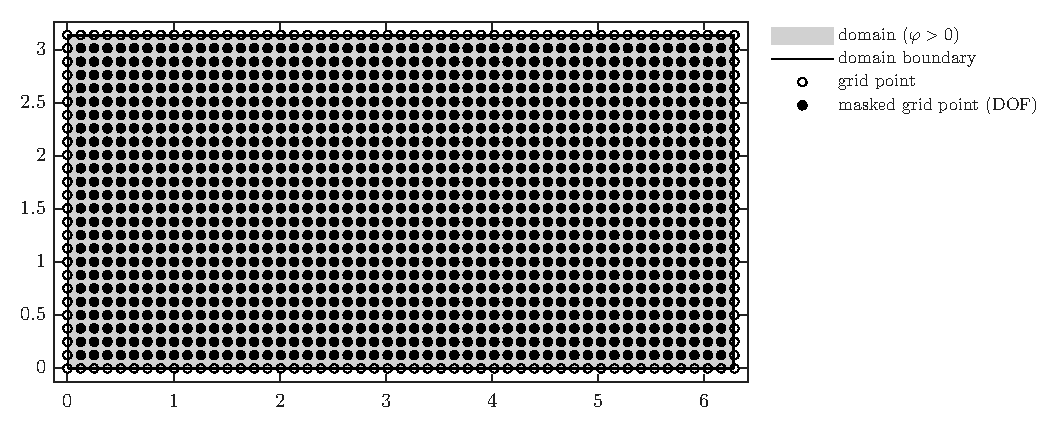
\includegraphics[width=0.4\textwidth]{rectangle_grid_M49_dofs1176}}
  \qquad
  \subfloat[Domain \texttt{ellipse\_minus\_quadrant}, $M = 47$, $\mathtt{DOF} = 649$.]{%
    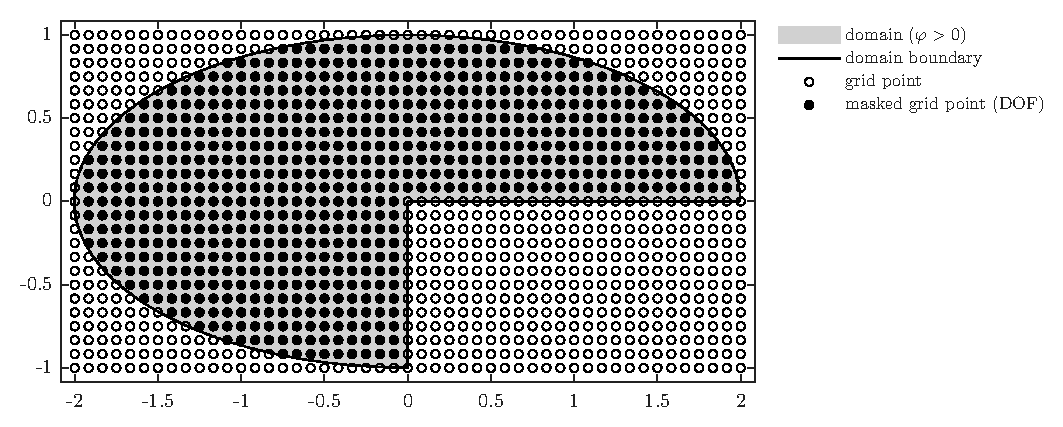
\includegraphics[width=0.4\textwidth]{ellipse_minus_quadrant_grid_M47_dofs649}}
  \\
  \subfloat[Domain \texttt{isosceles\_triangle}, $M = 50$, $\mathtt{DOF} = 1225$.]{%
    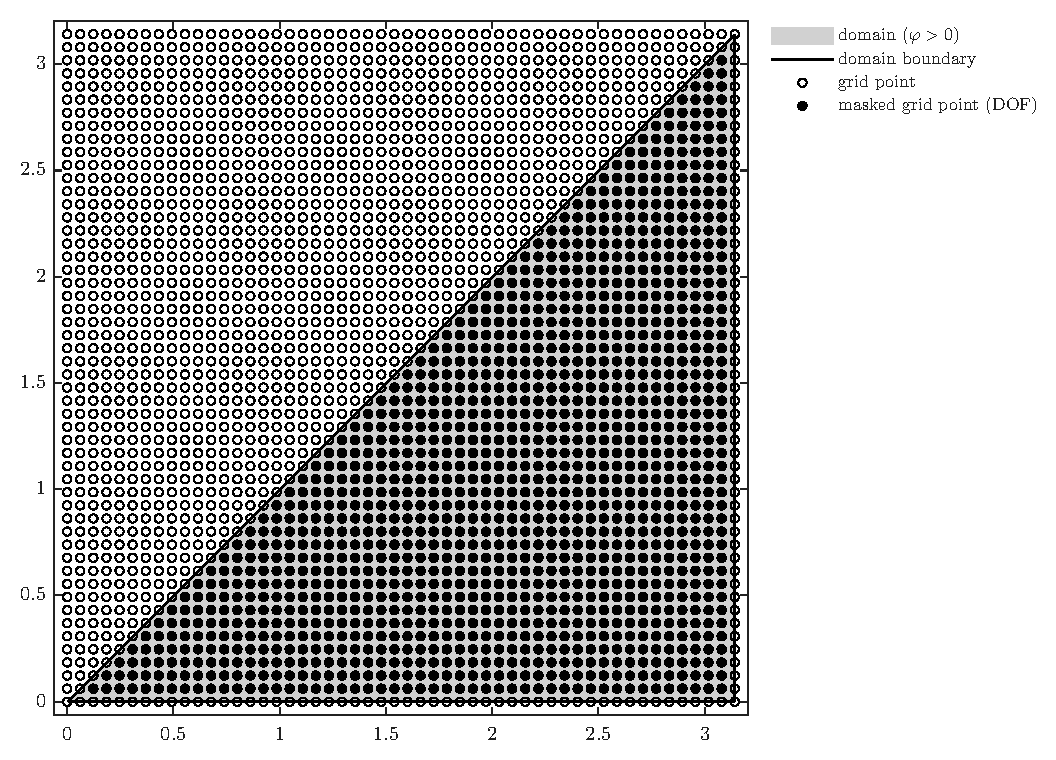
\includegraphics[width=0.4\textwidth]{isosceles_triangle_grid_M50_dofs1225}}
  \qquad
  \subfloat[Domain \texttt{L\_shaped}, $M = 49$, $\mathtt{DOF} = 1776$.]{%
    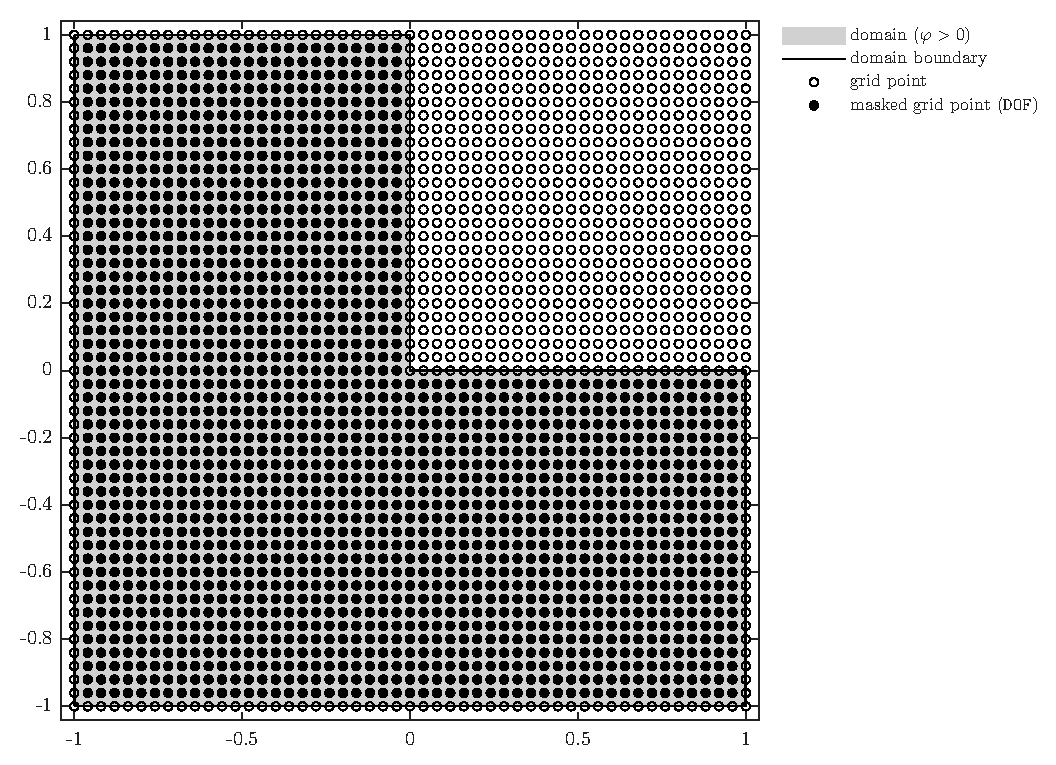
\includegraphics[width=0.4\textwidth]{L_shaped_grid_M49_dofs1776}}
  \\
  \subfloat[Domain \texttt{gww1}, $M = 50$, $\mathtt{DOF} = 936$.]{%
    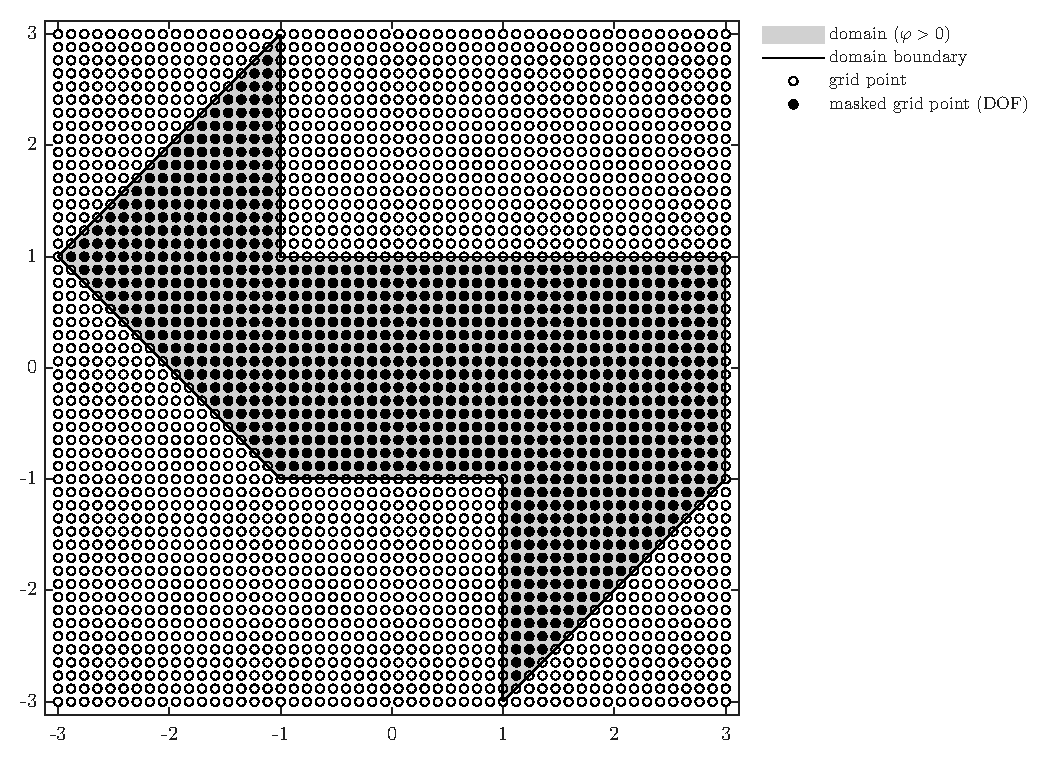
\includegraphics[width=0.4\textwidth]{gww1_grid_M50_dofs936}}
  \qquad
  \subfloat[Domain \texttt{gww2}, $M = 50$, $\mathtt{DOF} = 936$.]{%
    
\includegraphics[width=0.4\textwidth]{gww2_grid_M50_dofs936}}
  \\
  \subfloat[Domain \texttt{H\_shaped}, $M = 50$, $\mathtt{DOF} = 1888$.]{%
    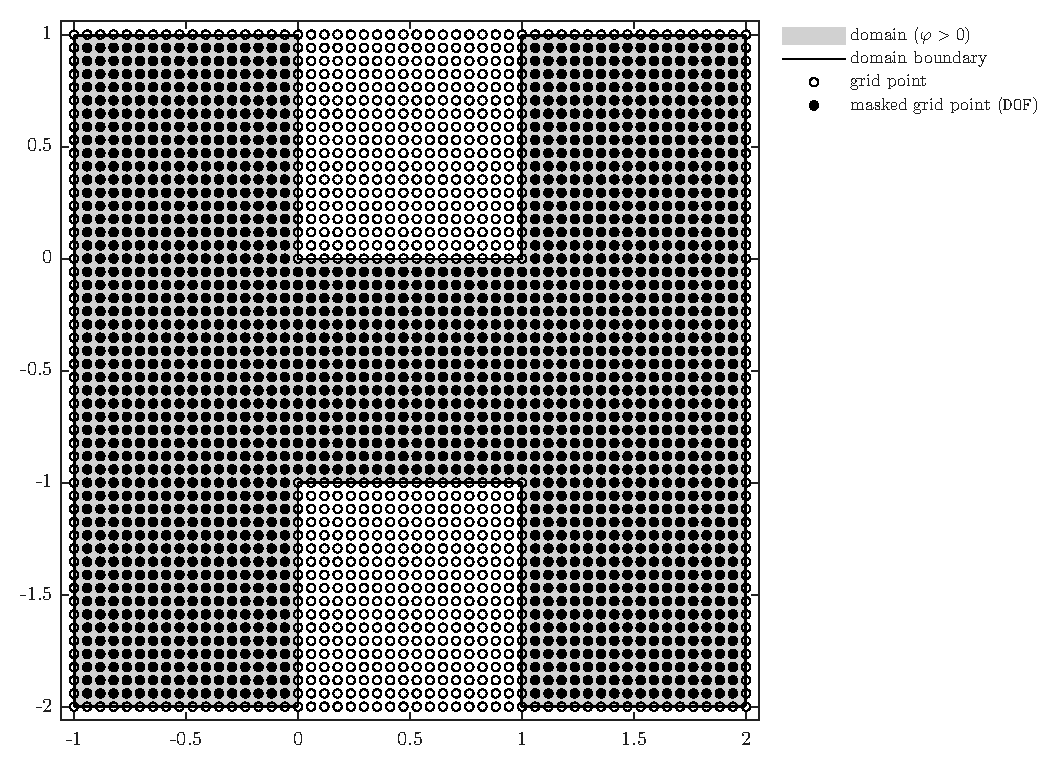
\includegraphics[width=0.4\textwidth]{H_shaped_grid_M50_dofs1888}}
  \caption{Visualisation of domains listed in Table~\ref{tab:domains_description} and sample grids for \texttt{DST} based discretisation.}
  \label{fig:domains}
\end{figure}
